\section{Motivating geometry in a matrix factorization model}
\label{sec:matrix-factorization}

Matrix factorization is a product model for nonlinear-moment geometry
\citep{kolda2009tensor,sidiropoulos2017tensor,anandkumar2014tensor}.
Following the motivating matrix-factorization application of
\citet{yamamoto2025hessianguided}, we study a regularized product-measure
extension and prove attraction along the anti-symmetric branch, transverse
descent, and positivity of the second variation along spherical product
pushforwards on an annulus and near the teacher. These population statements motivate the
positive--negative--positive curvature-response scenario, but do not construct
a connecting PWGF trajectory, transfer the second variations to the sampled
curvature \(\kappa_t^{Y,N}\), or verify its controlled-curvature path condition.

\subsection{Product-measure model}
\label{subsec:mf-model}

Let \(\mu=\mu_1\otimes\mu_2\) have marginals on \(\Sphere^{d_w-1}\),
and let \(z\sim N(0,I_{d_w})\).
For a vector-valued activation \(\sigma:\mathbb R\to\mathbb R^{d_h}\), define
the mean-field feature map
\(h_\nu(z):=\int\sigma(w^\top z)\,\nu(\dd w)\),
which averages features over weights \(w\sim\nu\).
Given a teacher \(\mu^o=\mu_1^o\otimes\mu_2^o\), consider
\begin{equation}
    F(\mu_1\otimes\mu_2)
    :=
    \frac12\E_z\left[
        \left\|h_{\mu^o_1}(z)h_{\mu^o_2}(z)^\top
        -h_{\mu_1}(z)h_{\mu_2}(z)^\top\right\|_{\mathrm F}^2
    \right]
    +
    \frac{\lambda_{\mathrm{reg}}}{p_W}Z_\pm(\mu_1,\mu_2)^{p_W/2},
    \label{eq:mf-objective}
\end{equation}
with \(\lambda_{\mathrm{reg}}>0\), \(p_W>2\),
\(\nu_\star^\pm:=\tfrac12\delta_{a_\star}+\tfrac12\delta_{-a_\star}\),
and \(Z_\pm(\mu):=Z_\pm(\mu_1,\mu_2):=\sum_{i=1}^2
W_{2,\Sphere}^2(\mu_i,\nu_\star^\pm)\), where
\(a_\star\in\Sphere^{d_w-1}\).
The spherical distance convention is given in
\Cref{subsec:product-spherical-model}.

\subsection{Branches and standing conditions}
\label{subsec:active-moments}

For \(0<r_{\mathrm{cap}}<\pi/2\), let \(\mathcal P_\pm(r_{\mathrm{cap}})\)
denote the class of probability measures whose closed supports lie inside
the two open spherical caps of radius \(r_{\mathrm{cap}}\) centered at
\(\pm a_\star\), with mass \(1/2\) in each cap.
Throughout this section, impose the following restrictions.
\begin{assumption}[Model restrictions; see \Cref{subsubsection:spherical-model-assumptions}]
\label{assumption:mf-model-restrictions}
\textbf{(i)} \(\mu_i,\mu_i^o\in\mathcal P_\pm(r_{\mathrm{cap}})\) for \(i=1,2\).
\textbf{(ii)} The nonzero Hermite coefficients of \(\sigma\) occur at a finite
set \(\mathcal O\) of odd degrees.
\textbf{(iii)} \(\mu_1^o=\mu_2^o=:\nu^o\).
\end{assumption}

For transverse descent in \Cref{prop:mf-local-geometry}\ref{item:mf-transverse-descent},
we additionally require a consistent average bias orthogonal to \(a_\star\)
across the two-sided latitude slices \(|a_\star^\top w|\), with a positive
margin away from the equator
(\Cref{assumption:quantitative-unweighted-two-sided-transverse-imbalance}).

Using standard Gaussian-input moment coordinates
\citep{arous2021online,abbe23a,bietti2023}, set
\(T_{i,n}:=\int w^{\otimes n}\mu_i(\dd w)\),
\(S_n:=(T_{1,n}+T_{2,n})/2\), and
\(A_n:=(T_{1,n}-T_{2,n})/2\) for \(n\in\mathcal O\).
Define
\begin{equation}
    \mathcal M_-:=\{\mu_1\otimes\mu_2:\mu_2=(-\Id)_\#\mu_1\},
    \qquad
    \mathcal M_+:=\{\mu_1\otimes\mu_2:\mu_1=\mu_2\}.
    \label{eq:branches}
\end{equation}
Membership in \(\mathcal M_-\) implies \(S_n=0\), and membership in
\(\mathcal M_+\) implies \(A_n=0\); the converses are not assumed.
The central target is \(\mu^\dagger:=\nu_\star^\pm\otimes\nu_\star^\pm\).

\begin{figure}
    \centering
    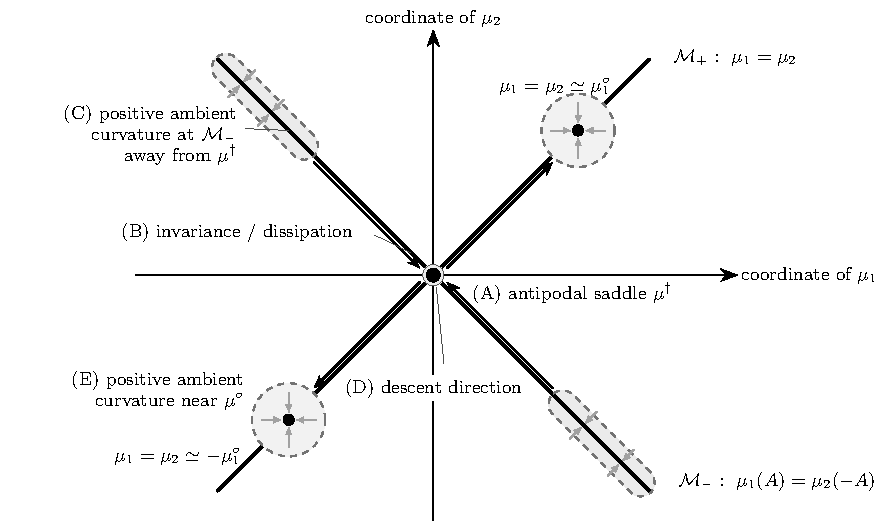
\includegraphics[width=0.7\linewidth]{sections/20260926-163335JST_eclair_transverse_arrows.pdf}
    \caption{Schematic local geometry in \Cref{prop:mf-local-geometry}: (A)--(B) the stationary target and its local attracting branch \ref{item:mf-local-attraction};
    (C) annular positive curvature \ref{item:mf-annular-curvature};
    (D) transverse descent \ref{item:mf-transverse-descent}; and
    (E) positive curvature near the teacher \ref{item:mf-teacher-curvature}.
    The diagram's \(-\mu_1^o\) denotes the reflected measure \((-\Id)_\#\mu_1^o\).
    Pale arrows depict curvature, not gradient-flow directions.
    The arrows do not assert a connecting trajectory.}
    \label{fig:eclair}
\end{figure}

\subsection{Local geometry}
\label{subsec:mf-curvature-pieces}

We use the spherical product pushforward second variation defined in
\Cref{lem:mf-full-spherical-Hessian}.
Admissible fields are smooth product tangent fields preserving the caps for
small perturbations; they need not be tangent to either branch. When the
prescribed pushforward path is a product Wasserstein geodesic, this second variation
is its usual geodesic second derivative.

\Needspace{5\baselineskip}
\begin{proposition}[Local geometry of the matrix factorization model]
\label{prop:mf-local-geometry}
Under \Cref{assumption:mf-model-restrictions}, with \(\lambda_{\mathrm{reg}}>0\) and \(p_W>2\), the following statements hold,
each under the additional conditions stated in its item.
\begin{enumerate}[label=(\roman*),ref=(\roman*),leftmargin=*]
\item \label{item:mf-local-attraction}
\textbf{Local attraction on the anti-symmetric branch (A--B).}
For \(2<p_W<3\), every globally well-posed characteristic product WGF in the sense of \Cref{def:mf-characteristic-solution} on
\(\mathcal M_-\) that starts sufficiently close to \(\mu^\dagger\) within the
cap class remains in that class and converges to \(\mu^\dagger\) in product
Wasserstein distance.
The precise initialization conditions and rate are given in
\Cref{prop:reduced-dissipation-antisymmetric-branch}.

\item \label{item:mf-annular-curvature}
\textbf{Positive ambient curvature on an annulus (C).}
For every \(\zeta_->0\), if \(\lambda_{\mathrm{reg}}\) is sufficiently large,
depending on \(\zeta_-\) and the fixed model parameters, then at every
\(\mu\in\mathcal M_-\) with \(Z_\pm(\mu)\ge\zeta_-^2\), the spherical product
pushforward second variation is positive in every nonzero admissible direction.
The quantitative threshold and lower bound are given in
\Cref{cor:branchwise-positivity-Wasserstein-Mminus}.

\item \label{item:mf-transverse-descent}
\textbf{Transverse descent at the target (D).}
If \(\mathcal O\ne\varnothing\) and the teacher satisfies
\Cref{assumption:quantitative-unweighted-two-sided-transverse-imbalance}
at \(a_\star\), ensuring a non-cancelling transverse teacher signal,
there exists a same-density transverse perturbation \(\mu_h\) from
\(\mu^\dagger\) such that, as \(h\to0\),
\(F(\mu_h)=F(\mu^\dagger)-\gamma_{\mathrm{esc}}h^2+o(h^2)\),
with \(\gamma_{\mathrm{esc}}>0\).
Its construction is given in
\Cref{lemma:descent-direction-antipodal-dirac-from-unweighted-imbalance}.
The regularizer contributes \(O(|h|^{p_W})=o(h^2)\).

\item \label{item:mf-teacher-curvature}
\textbf{Positive ambient curvature near the teacher (E).}
If \(Z_\pm(\mu_+^o)>0\), where \(\mu_+^o:=\nu^o\otimes\nu^o\),
the spherical product pushforward second variation has a positive uniform
margin in a sufficiently
small product Wasserstein neighborhood of \(\mu_+^o\), relative to the cap class.
The existence of the margin and neighborhood is proved in
\Cref{prop:Mplus-teacher-local-positive-curvature}.
The teacher need not be stationary for the regularized objective.
\end{enumerate}
\end{proposition}
